%% Options:
\documentclass[
% twocolumn,
% hf,
]{ceurart}

\sloppy

\usepackage{listings}

\lstset{breaklines=true}

\begin{document}

\copyrightyear{2022}
\copyrightclause{Copyright for this paper by its authors.
  Use permitted under Creative Commons License Attribution 4.0
  International (CC BY 4.0).}

\conference{Ontology Alignment Evaluation Initiative (OAEI) 2022 campaign, October 23rd or 24th, 2022, Hangzhou, China}

\title{Cross-lingual ontology matching with CIDER-LM: results for OAEI 2022}

\author{Javier Vela}[%
orcid=0000-0002-6818-9191,
email=775593@unizar.es,
url=https://github.com/javiervela/,
]
\author{Jorge Gracia}[%
orcid=0000-0001-6452-7627,
email=jogracia@unizar.es,
url=http://jogracia.url.ph/web/,
]

\address{Department of Computer Science and Systems Engineering\\ University of Zaragoza \\
María de Luna 1, 50018 Zaragoza, Spain}

% REVIEW2 minor grammatical corrections and improvements (by Writefull tool)

\begin{abstract}
In this paper, the CIDER-LM cross-lingual matching system is presented, as well as the results it achieved during the OAEI (Ontology Alignment Evaluation Initiative) 2022 campaign. This is the first appearance of CIDER-LM in OAEI where it only participated in MultiFarm, the track for cross-lingual ontology alignment evaluation. The matching system uses a pre-trained multilingual language model based on transformers, fine-tuned using the openly available portion of the MultiFarm dataset. The model calculates the vector embeddings of the labels associated to every ontology entity and its context. The confidence degree between matching entities is computed as the cosine similarity between their associated embeddings. CIDER-LM is novel in the use of multilingual language models for cross-lingual ontology matching. Its initial version obtained promising results in the OAEI'22 MultiFarm track, attaining a modest precision but the best overall performance in recall. 
\end{abstract}

\begin{keywords}
    Cross-lingual Ontology Matching \sep
    Ontology Alignment \sep
    Natural Language Processing \sep
    Language Models \sep
    Transformers \sep
    CIDER-LM \sep
    Sentence-BERT
\end{keywords}

\maketitle

\section{Presentation of the system}

CIDER-LM is largely inspired by an earlier system called CIDER-CL~\cite{Gracia2013cidercl}, the cross-lingual version of CIDER (Context and Inference basED ontology alignER), although CIDER-LM completely redesigns and reimplements it. CIDER-LM stands for Language Model-based CIDER. Unlike its predecessor, which based its cross-lingual capabilities on \textit{cross-lingual explicit semantic analysis}~\cite{Sorg2012}, CIDER-LM uses \textit{language models} as BERT~\cite{Devlin2019} based on the Transformer architecture~\cite{Vaswani2017}. Transformers are encoder-decoder neural networks with a self attention mechanism. They are very popular for solving \textit{Natural Language Processing} (NLP) tasks. 
BERT is a language model that leverages the transformer encoder to predict tokens in a sentence when given a context. Numerous studies have been published exploring how BERT can be fine-tuned to solve a wide variety of NLP tasks. The original BERT was pre-trained using a document-level corpus in English, extracted from the BooksCorpus\footnote{\url{https://huggingface.co/datasets/bookcorpus}} (800M words) and the English Wikipedia\footnote{\url{https://huggingface.co/datasets/wikipedia}} (2,500M words).

% REVIEW2: 2nd sentence to the end l.57 : removec "; and recently, tasks from other fields, such as computer vision."
% Because BERT is not used for Computer Vision, rather the Transformers arquitecture, as far as I know

The use of BERT and similar models has proven to be useful in ontology matching, for example, in the biomedical domain~\cite{He2021}, but they have been largely unexplored for cross-lingual matching until now. Multilingual language models can be used to that end, which can represent tokens in several languages in the same embedding space.

%, but other BERT variants have been trained to cover other languages. %BERT also has proven to be useful in the translation task between two languages predetermined in the training phase. 

Sentence-BERT (SBERT)~\cite{Reimers2019}, which is a modification of the pre-trained BERT, produces semantically meaningful embeddings for sentences. These sentence embeddings are aligned in the same embedding space, in contrast to other models that create the embeddings at the token level. In addition, SBERT monolingual models can be made multilingual using \textit{knowledge distillation}~\cite{reimers-2020-multilingual-sentence-bert}. The resulting models produce vector embeddings that can be compared to find the similarity between sentences in two different languages.

% In fact, other BERT variants have been trained with multilingual corpora. One of such a variants, Sentence-BERT (SBERT)~\cite{Reimers2019}, produces semantically meaningful embeddings for sentences in different languages, which are aligned in the same embedding space (in contrast to other models that create the embeddings at the token level). These aligned embeddings can be compared to find the similarity between sentences in two different languages. % CIDER-LM uses SBERT, which computes semantically meaningful sentence embeddings and, compared to BERT, reduces the time for comparing between the embeddings using the \textit{cosine similarity}. 
% In addition, SBERT monolingual models can be made multilingual using \textit{knowledge distillation}~\cite{reimers-2020-multilingual-sentence-bert}.

% REVIEW2 !! TODO !! beginning l.66: SBERT is not only multilingual, so the additional citation makes sense in the multilingual context. May require further rephrasing

% REVIEW2: end l.69 add citation

CIDER-LM uses SBERT to associate embeddings to the labels of the ontology entities (and their context), which are compared using cosine similarity to create a matching confidence score between them. The choice of sentence embeddings instead of token embeddings (as other multilingual language models do) is motivated by the fact that many ontology labels are conformed by multi-word expressions, thus embeddings that represent whole sentences (and not only atomic tokens) are more suitable to capture their semantic content and to compute similarities between them~\cite{Neutela2021, Reimers2019}.

\subsection{State, purpose, general statement}

CIDER-LM is a cross-lingual ontology matching system that utilizes a transformer-based pre-trained multilingual language model, fine-tuned using the openly available portion of the MultiFarm dataset\footnote{\url{https://www.irit.fr/recherches/MELODI/multifarm/}}. The model calculates the vector embeddings of the labels associated to
every ontology entity and its context. The confidence degree between two matching entities is computed as
the cosine similarity between their associated embeddings.
The generated alignments are one-to-one mappings between entities from two input ontologies. The input ontologies must be in OWL or RDF-S format, and the output provided is expressed in Alignment Format\footnote{\url{http://alignapi.gforge.inria.fr/format.html}}. The type of discovered correspondence is ``equivalence", with a confidence degree in $[0,1]$. CIDER-LM works with ontology classes and properties, not yet with instances.

\subsection{Specific techniques used}

CIDER-LM integrates a fine-tuned version of \textit{distiluse-base-multilingual-cased-v2}\footnote{\url{https://huggingface.co/sentence-transformers/distiluse-base-multilingual-cased-v2}}, a multilingual pre-trained model from Sentence Transformers\footnote{\url{https://www.sbert.net/docs/pretrained_models.html##multi-lingual-models}}.
This ontology aligner is implemented in Python and is wrapped using the \textit{Matching EvaLuation Toolkit} (MELT), a framework for ontology matching and evaluation~\cite{Hertling2019melt}. The system is packaged as a Docker image implementing the \textit{Web Interface}\footnote{\url{https://dwslab.github.io/melt/matcher-packaging/web##web-interface-http-matching-interface}}. 

An overall view of the CIDER-LM matching pipeline is shown in Figure \ref{fig:architecture}. In short, the process is as follows. First, the aligner receives a source ($O_1$) and target ($O_2$) ontology. Both ontologies are read into Python objects using the library Owlready2\footnote{\url{https://owlready2.readthedocs.io/en/v0.37/}} and fed individually into a semantic reasoner, which extends the ontologies by inferring semantic relations not initially declared. The classes and properties labels extracted from both ontologies are verbalized using their ontological context. Then, the verbalized labels are passed to the Transformer model that obtains an embedding for each of the entities in the ontologies (i.e., a vector capturing the semantics of the entity). Each embedding from $O_1$ is compared to every embedding from $O_2$ using cosine similarity, forming a bipartite graph. The Maximum Weight Bipartite Extractor algorithm obtains an initial alignment that is reduced by a threshold filter, obtaining the final alignment. The following paragraphs describe each of the involved techniques with some more detail.

\begin{figure}
  \centering
  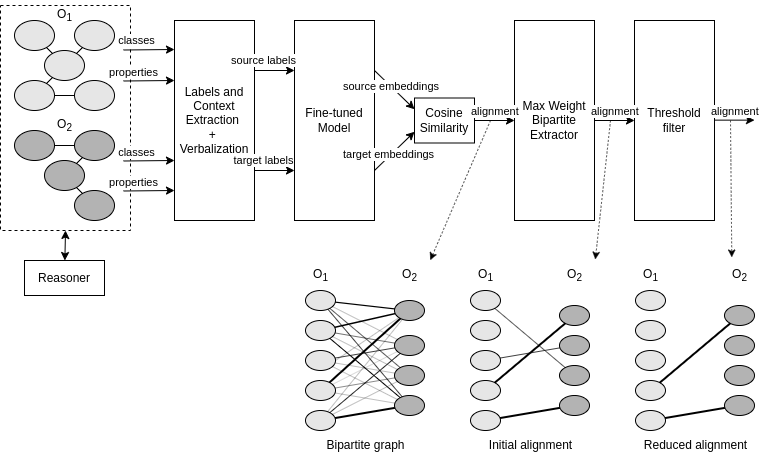
\includegraphics[width=\linewidth]{cider-lm-architecture-3.drawio.png}
  \caption{CIDER-LM architecture: Given two ontologies $O_1$ and $O_2$, they are expanded by a reasoner. The labels characterising the compared entities are extracted, verbalized, and an embedding is obtained for every one of them. The embeddings are compared using the Cosine Similarity, passed through the Max Weight Bipartite Extractor and the Threshold Filter, obtaining the final alignment.}
  \label{fig:architecture}
\end{figure}


\subsubsection{Ontology Reasoning}

CIDER-LM performs a preliminary reasoning of both the source and the target ontologies using HermiT OWL Reasoner\footnote{\url{http://www.hermit-reasoner.com/}}. This step expands the semantic relations in the ontologies, inferring new knowledge not initially asserted. However, including the reasoning in the pipeline increases the execution time of CIDER-LM considerably. This step is optional, but we kept it for OAEI-22.  

\subsubsection{Verbalization of entities}
CIDER-LM considers ontology classes and properties. For both types of entities, their associated labels are extracted to build the corresponding sentence embeddings. 
In order to make the calculated embedding more representative of the semantics of the analyzed ontology entity, the labels of other entities that are part of its ontological context are considered. The verbalization process is needed so that the language model can process the set of labels (coming from the entities and its ontological context) as an individual sentence.

%The purpose of extending the label (verbalization) is to include the hierarchical information (for classes), and domain and range information (for properties) in the final embedding used on the calculation of the matching confidences. CIDER-LM obtains the labels of the neighboring entities from the ontology after the reasoning.
In its current version, CIDER-LM builds the ontological context of an entity based on its neighboring entities, treating classes and properties differently (we use `+' as the string concatenation operator):

\textbf{Class Verbalization}. For a class $a$ and its label $l(a)$, the set of parent classes and child classes in the hierarchy of the ontology are $P_a$ and $C_a$, respectively. The verbalization of the class is the concatenation of the following:

\begin{itemize}
    \item $l(a)$ + `\verb|, |' ;
    \item for every class in $P_a$: $l(a)$ + `\verb| is a |' + $l(P_a^i)$ + `\verb|, |' 
    \item for every class in $C_a$: $l(C_a^i)$ + `\verb| is a |' + $l(a)$ + `\verb|, |' 
\end{itemize}

\textbf{Property Verbalization}. For a property $a$ and its label $l(a)$, the sets of its domain and range classes in the ontology are $D_a$ and $R_a$, respectively. The verbalization of the property is the concatenation of the following:

\begin{itemize}
    \item $l(a)$ + `\verb|, |' 
    \item for every entity in $D_a$: $l(a)$ + `\verb| has domain |' + $l(D_a^i)$ + `\verb|, |' 
    \item for every entity in $R_a$: $l(a)$ + `\verb| has range |' + $l(R_a^i$) + `\verb|, |' 
\end{itemize}

Supposing that a certain entity has more than one label assigned, the first label is chosen to concatenate in the verbalization.
The verbalized sentences from labels are concatenated with particles in English, independently of the language of the ontology. During the preliminary evaluation of the system, we found evidence that the particular language used for concatenating the labels was not very relevant, even if it differed from the language of the ontology. This will require further exploration in the future. %used and whether it matches the ontology language is barely relevant.

%\subsubsection{Transformer-based Multilingual Language Models}
%MOVIDO ARRIBA Y A LA SECCION DE FINE_TUNING

%\subsubsection{Cosine Similarity}

%The \textit{Cosine-Similarity} is a metric employed to find the distance between two number sequences, vectors. It is the cosine between the embeddings obtained from the sentences in the embedding space, and is a measure of how similar two sentences (the entity labels) are. The \textit{Cosine-Similarity} is used as the confidence of a match between two entities. 

\subsubsection{Fine-tuned language model}

%% REVIEW ::: 512 dimensional dense vector space (end l.143)

% CIDER-LM computes the similarity between two labels using \verb|distiluse-base-multilingual-cased-v2|, which is a pre-trained multilingual model trained using the SBERT architecture. 

 CIDER-LM relies on \verb|distiluse-base-multilingual-cased-v2|, which is pre-trained on Semantic Textual Similarity (STS) and uses the SBERT architecture. The model is the knowledge-distilled version of the Universal Sentence Encoder and supports more than 50 languages. Given a sentence, the model obtains a vector embedding in a  512 dimensional dense vector space.
 A checkpoint of the \verb|distiluse-base-multilingual-cased-v2| model has been downloaded from HuggingFace, using the \textit{SentenceTransformers} Python framework.

 %REVIEW-2 (end l. 154) remove " and fine-tuned for CIDER-LM"
 % It says on the next paragraph, right away
 
 In fact, CIDER-LM uses a fine-tuned version of the model, specialized on the task of obtaining similarities between two entity labels in different languages. Given a set of pairs of entity labels obtained from the training set and a \textit{true confidence} of $1$ or $0$, indicating if the entities are a match or not; the model is trained on reducing the \textit{CosineSimilarityLoss} between the \textit{predicted} and \textit{true confidence}. We use the \textit{SenteceTransformers} framework and a basic training pipeline to obtain the fine-tuned model used on the matching system. 

The \textit{cosine similarity} metric is used to find the distance between the vector embeddings associated with the entities that come from the two different ontologies in the common embedding space. This offers a measure of how similar two sentences (the verbalised sets of entity labels) are, resulting in the confidence degree associated to the possible matching between the two entities. 

\subsubsection{Maximum Weight Bipartite Extractor}

CIDER-LM obtains the matching confidence for every pair of entities from the target and source ontology. Once the confidence degrees have been determined, the alignment can be considered as a bipartite graph with an edge (the confidence in a match) from every node (entity) from the source ontology to the target ontology. Using the implementation of the Hungarian algorithm in the \textit{scipy}\footnote{\url{https://scipy.org/}} Python library, the maximum weight matching in bipartite graphs problem is solved. 

\subsubsection{Threshold filter}

After having a complete alignment, a threshold filter is used to remove all the correspondences with low confidence from the alignment. Every correspondence with a confidence lower than the default threshold value is removed. The threshold value can be used to direct the results obtained by the system: a higher value will promote precision, while a lower value will favour recall. CIDER-LM applies a default threshold value of $0.5$ that, according to the results, promotes recall.

\subsection{Adaptations made for the evaluation}

To participate in the OAEI campaign, we have wrapped the Python implementation of CIDER-LM around the \verb|MatcherCLI| Java class from the MELT framework. Wrapping enables MELT evaluation and the packaging plugin, which is used to create the Docker container image for submission to the OAEI.

CIDER-LM performs a preliminary substitution of `\verb|&xsd;date|' for `\verb|&xsd;dateTime|' and `\verb|http://www.w3.org/2001/XMLSchema#date|' for `\verb|http://www.w3.org/2001/XMLSchema#dateTime|' because the dataset of ontologies used for the evaluation was not initially recognized by the HermiT reasoner as OWL Version 2, which is the only version of the format taken by the reasoner. Performing the substitution fixes the error reading the ontology.

\subsection{Link to the system and parameters file}\label{sec:system-link}

The implementation of the system is hosted in a GitHub repository\footnote{\url{https://github.com/sid-unizar/CIDER-LM}}. The container image with the matching system is also available on GitHub in the \textit{Packages} section. 

\section{Results}

In its first participation in the OAEI campaign (2022), CIDER-LM contributed to the MultiFarm track only. The reason is that this tool is primarily aimed at cross-lingual ontology matching. However, the method is able to produce monolingual mappings as well, so we do not discard participation in other tracks in future OAEI editions. 

The MultiFarm evaluation involves two ontologies from the Conference domain (edas and ekaw), which are translated into eight languages from English, resulting in 55 x 24 matching tasks.
Details about the test ontologies, the evaluation process, and the complete results for the MultiFarm track can be found on the OAEI'22 website\footnote{\url{https://oaei.ontologymatching.org/2022/multifarm/index.html}}.
%\subsection{MultiFarm}
The results reported by the OAEI organisers on October 9th of 2022 describe the precision, recall and F-measure of the alignments produced by each of the participant systems. The aggregated results for completing the matching task are shown in Table \ref{tab:multifarm-results}.

\begin{table*}
	\caption{MultiFarm aggregated results per matcher for different ontologies}
	\label{tab:multifarm-results}
	\begin{tabular}{lcccc}
	  \toprule
	  System & Time(Min) & Precision & F-measure & Recall\\
	  \midrule
	   CIDER-LM             & $\sim 157$ & 0.16    			& 0.25     			& \textbf{0.58}    \\
	   LSMatch              & $\sim 33$  & 0.24    			& 0.038    			& 0.021            \\
	   LSMatch Multilingual & $\sim 69$  & 0.68    			& \textbf{0.47}     & 0.36             \\
	   LogMap               & $\sim 9$   & \textbf{0.72}    & 0.44     			& 0.31             \\
	   LogMapLt             & $\sim 175$ & 0.24    			& 0.038    			& 0.02             \\
	\bottomrule
  \end{tabular}
  \end{table*}

% REVIEW update results. Remove Matcher (remove l.192)

\section{General comments}

The following sections contain some remarks and comments on the results obtained and the evaluation process.

\subsection{Comments on the results}

The obtained results in MultiFarm are intermediate in terms of F-measure (third-best result out of five participants), and are also very good in terms of recall, having attained the best result of any OAEI edition for the MultiFarm ``different ontologies" sub-task\footnote{Only in OAEI'12 higher values can be found, but from two matchers that gave nearly every possible combination as result, thus resulting in close to zero values of precision and F-measure}.

The results of CIDER-LM largely improve those obtained by its predecessor tool CIDER-CL~\cite{Gracia2013cidercl} for the MultiFarm different ontologies subtask, which were $P = 0.16$, $R = 0.19$, and $F = 0.17$

The results of CIDER-LM in the OAEI multilingual track are still modest, especially in precision, but the fact that even the best systems do not score very high illustrates the difficulty of the problem. For instance, the F-measure attained in MultiFarm was never higher than 0.47 in any OAEI edition.  

\subsection{Discussions on the way to improve the proposed system}

The analysis of the OAEI'22 results shows that the CIDER-LM matching system has the potential to improve its current results in several ways. For instance, the current version builds embeddings based on the entity labels, the labels of parents and children for classes, and the labels of domain and range for properties. A future version could include more features in the verbalization of labels. 

The current results show a clear unbalance between precision and recall. A higher threshold value would help promote the precision measure, further achieving a higher F-measure. The results also show that the execution time of the tool is greater than that of the other participants. Removing the use of a reasoner would greatly reduce the time, with only a small impact on the performance of the results, as seen in our internal experiments.

Furthermore, a more careful study of the fine-tuning process could lead to an improvement of the CIDER-LM alignment results. Involving more sophisticated techniques on the training and validation of the fine-tuned model can reduce overfitting and provide a more general model that behaves better with ontologies different from the ones seen in training.

%At last, we would like to use the MELT Transformers extension to implement the system to achieve a more reusable implementation of the tool that is better adjusted with the OAEI standards. A Java system was not implemented for the 2022 campaign due to the little familiarity with MELT and its learning curve being greater than Python.

\subsection{Comments on the OAEI procedure}

The MELT wrapper for the Python matching system has proven to be easy to comprehend and implement, and useful for encapsulating the tool and later creating the web server container image for the OAEI submission. We consider the inclusion of the MELT framework a significant advancement in OAEI to allow the integration and participation of non-Java-based implementations.

\section{Conclusion}

This paper presented the first version of CIDER-LM, which explores for the first time the potential of multilingual language models on the task of finding cross-lingual alignments between ontologies in different languages. %The system obtains the confidences of the alignment using a transformer-based multilingual language model. 
The system uses SBERT, a multilingual language model based on the Transformer architecture. It was evaluated on the OAEI'22 MultiFarm track, achieving intermediate results in terms of the F-measure and very good results in terms of recall. Although there is much room for further improvements, we consider that CIDER-LM results have proved the viability of using multilingual language models for this task. 

In future versions, more features will be considered to build the ontological context, new verbalization strategies will be analyzed, and a more careful study of the fine-tuning process will be carried out, to attain a better and more general model for cross-lingual ontology matching.

\begin{acknowledgments}

This article is the result of a collaboration grant 2021-22 at the Department of Computer Science and Systems Engineering, University of Zaragoza, funded by the Ministry of Education and Professional Training (Spain). It has also been partially supported by the Engineering Research Institute of Aragon (I3A), by the Spanish project PID2020-113903RB-I00 (AEI/FEDER, UE), by DGA/FEDER, and by the {\em Agencia Estatal de Investigación} of the Spanish Ministry of Economy and Competitiveness and the European Social Fund through the ``Ramón y Cajal'' program (RYC2019-028112-I).

%% REVIEW add I3A (end l.233)

\end{acknowledgments}

\bibliography{cider-lm}

\end{document}

%%
%% End of file